\documentclass[11pt]{article}

\usepackage{classDM17}
\usepackage{hyperref}
\usepackage{float}
\usepackage[normalem]{ulem}
\usepackage{listings}

\newcommand{\norm}[1]{\left|\left| #1 \right|\right|}

\title{Assignment 5: Regression}
\author{Christohper Mertin/\verb~u1010077~\\
        \url{cmertin@cs.utah.edu}}
\date{\today}



\begin{document}
\maketitle

%\end{titlepage}




%%%%%%%%%%%%%%%%%%%%%%%%%%%%%%%%%%%%%%%%%%%%%%%%%%%%
%%%%%%%%%%%%%%%%%%%%%%%%%%%%%%%%%%%%%%%%%%%%%%%%%%%%
%%%%%%%%%%%%%%%%%%%%%%%%%%%%%%%%%%%%%%%%%%%%%%%%%%%%
\section*{Overview}

In this assignment you will explore regression techniques on high-dimensional data.  

You will use a few data sets for this assignment:
\begin{itemize} \denselist
\item \href{http://www.cs.utah.edu/~jeffp/teaching/cs5140/A5/A.dat}{\texttt{http://www.cs.utah.edu/\~{}jeffp/teaching/cs5140/A5/A.dat}}
\item \href{http://www.cs.utah.edu/~jeffp/teaching/cs5140/A5/X.dat}{\texttt{http://www.cs.utah.edu/\~{}jeffp/teaching/cs5140/A5/X.dat}}
\item \href{http://www.cs.utah.edu/~jeffp/teaching/cs5140/A5/Y.dat}{\texttt{http://www.cs.utah.edu/\~{}jeffp/teaching/cs5140/A5/Y.dat}}
\item \href{http://www.cs.utah.edu/~jeffp/teaching/cs5140/A5/M.dat}{\texttt{http://www.cs.utah.edu/\~{}jeffp/teaching/cs5140/A5/M.dat}}
\item \href{http://www.cs.utah.edu/~jeffp/teaching/cs5140/A5/W.dat}{\texttt{http://www.cs.utah.edu/\~{}jeffp/teaching/cs5140/A5/W.dat}}
\end{itemize}
and a file stub:
\begin{itemize} \denselist
\item \href{http://www.cs.utah.edu/~jeffp/teaching/cs5140/A5/FD.m}{\texttt{http://www.cs.utah.edu/\~{}jeffp/teaching/cs5140/A5/FD.m}}
\end{itemize}

These data sets are in matrix format and can be loaded into MATLAB or OCTAVE.  By calling 
\\
\texttt{load filename} (for instance \texttt{load X.dat})
\\
it will put in memory the data in the file, for instance in the above example the matrix \texttt{X}.  You can then display this matrix by typing 

\texttt{X}

\vspace{.1in}

\emph{As usual, it is highly recommended that you use LaTeX for this assignment.  If you do not, you may lose points if your assignment is difficult to read or hard to follow.  Find a sample form in this directory:
\url{http://www.cs.utah.edu/~jeffp/teaching/latex/}}


%%%%%%%%%%%%%%%%%%%%%%%%%%%%%%%%%%%%%%%%%%%%%%%%%%%%
%%%%%%%%%%%%%%%%%%%%%%%%%%%%%%%%%%%%%%%%%%%%%%%%%%%%
%%%%%%%%%%%%%%%%%%%%%%%%%%%%%%%%%%%%%%%%%%%%%%%%%%%%
\section{Singular Value Decomposition (20 points)}

First we will compute the SVD of the matrix \texttt{A} we have loaded

\noindent
\texttt{[U,S,V] = svd(A)}

Then take the top $k$ components of \texttt{A} for values of $k = 1$ through $k=10$ using

\noindent
\texttt{Uk = U(:,1:k)}
\\ \noindent
\texttt{Sk = S(1:k,1:k)}
\\ \noindent
\texttt{Vk = V(:,1:k)}
\\ \noindent
\texttt{Ak = Uk*Sk*Vk'}

\paragraph{A (10 points):}
Compute and report the $L_2$ norm of the difference between \texttt{A} and \texttt{Ak} for each value of $k$ using

\noindent
\texttt{norm(A-Ak,2)}

\begin{figure}[H]
\centering
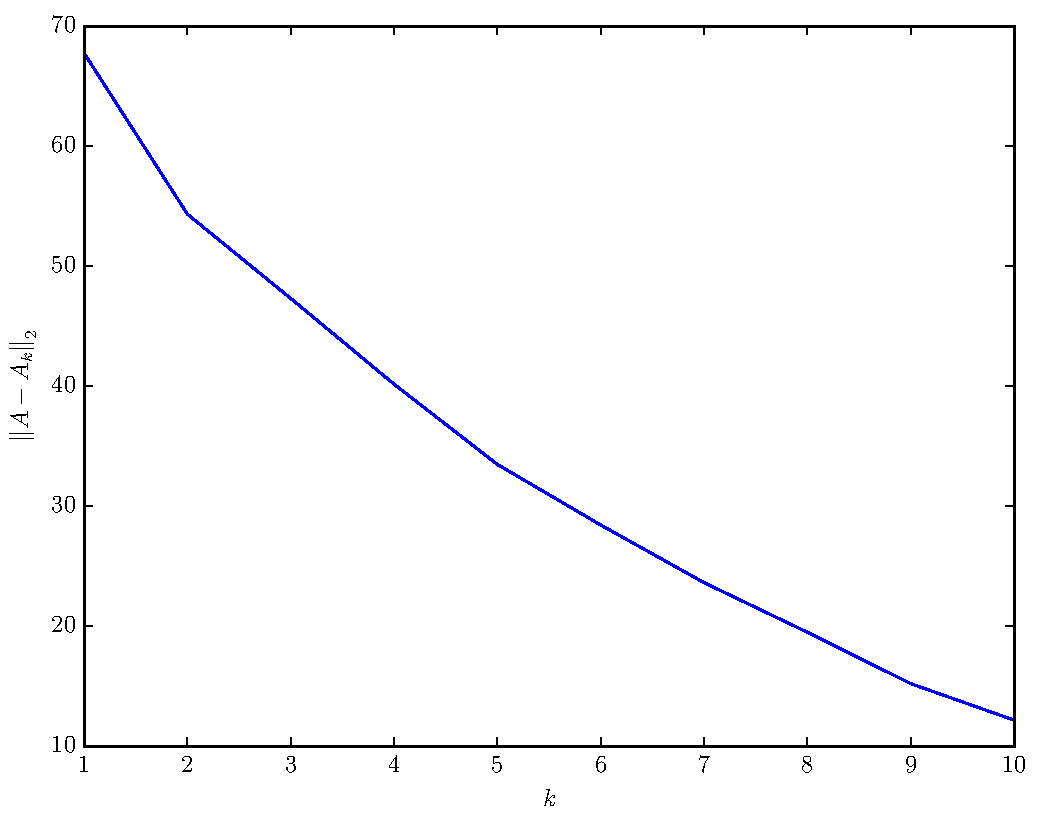
\includegraphics[width=.75\textwidth]{prob1a.pdf}
\end{figure}

\paragraph{B (5 points):}
Find the smallest value $k$ so that the $L_2$ norm of \texttt{A-Ak} is less than 10\% that of \texttt{A}; $k$ might or might not be larger than $10$.  

\verb~Minimum k:  10~

\paragraph{C (5 points):}
Treat the matrix as 1125 points in 30 dimensions.  Plot the points in $2$ dimensions in the way that minimizes the sum of residuals squared.  

PCA allows us to map down to a lower dimensional space from $\mathbb{R}^{d}$ to $\mathbb{R}^{k}$ by selecting the first $k$ significant right singular vectors. This only works if the data is can be reprsented in Euclidean space, but it is assumed so for this problem. The plot of the data can be seen below, where the first two largest singlar vectors were chosen as the $x$ and $y$ to plot the data.

\begin{figure}[H]
\centering
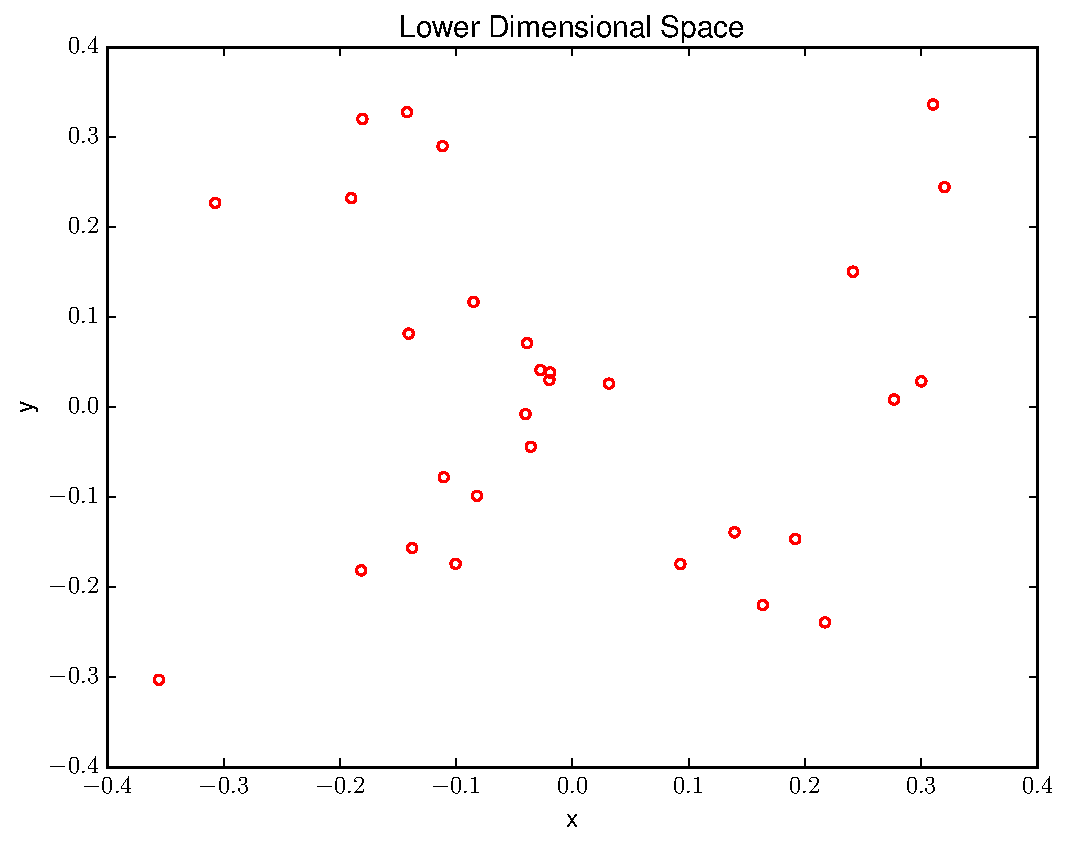
\includegraphics[width=.75\textwidth]{lower_dim.pdf}
\end{figure}



%%%%%%%%%%%%%%%%%%%%%%%%%%%%%%%%%%%%%%%%%%%%%%%%%%%%
%%%%%%%%%%%%%%%%%%%%%%%%%%%%%%%%%%%%%%%%%%%%%%%%%%%%
%%%%%%%%%%%%%%%%%%%%%%%%%%%%%%%%%%%%%%%%%%%%%%%%%%%%
\section{Frequent Directions and Random Projections (40 points)}

Use the stub file $\texttt{FD.m}$ to create a function for the Frequent Directions algorithm (\textbf{Algorithm 15.2.1}).  We will consider running this code on matrix \texttt{A}.  

\paragraph{A (20 points):}
We can measure the error $\max_{\|x\|=1} | \|A x\|^2 - \|B x\|^2 |$ as 
\texttt{norm(A'*A - B'*B, 2)}.  
\begin{itemize} \denselist
\item How large does \texttt{l} need to be for the above error to be at most $\|A\|_F^2 /10$?  

\verb~Minimum l:  10~

\item How does this compare to the theoretical bound (e.g. for $k=0$).

\begin{figure}[H]
\centering
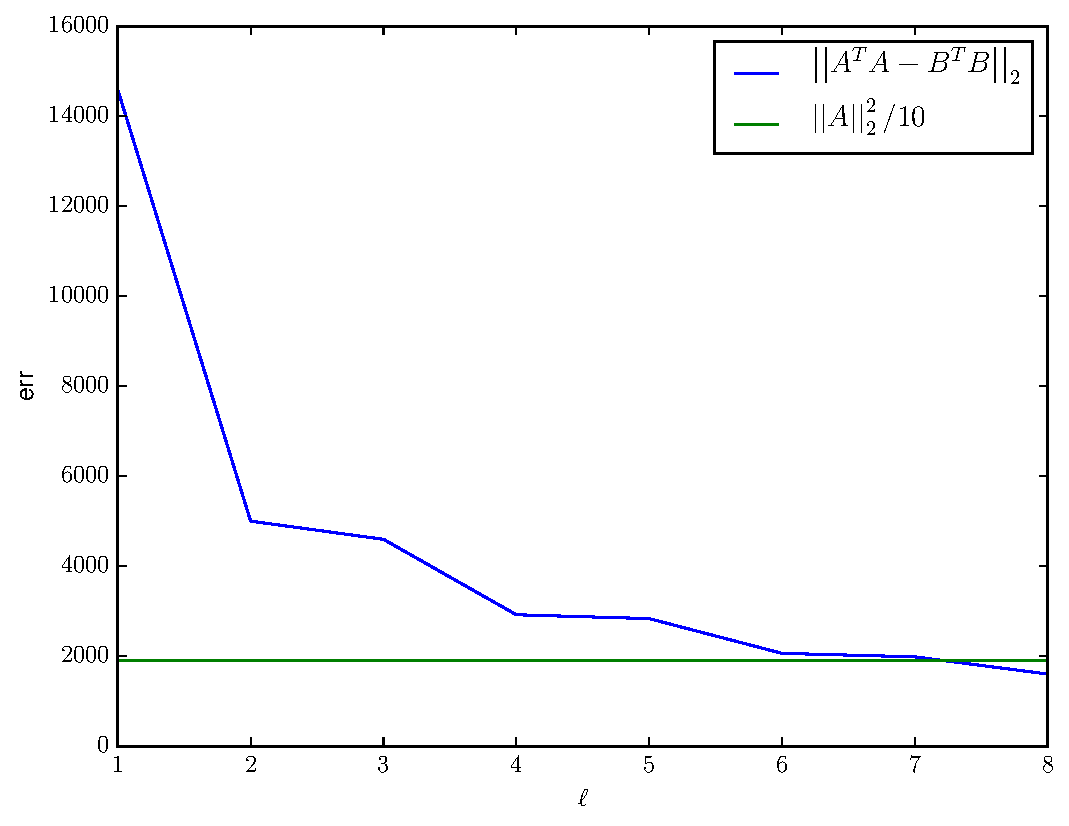
\includegraphics[width=.75\textwidth]{prob2a.pdf}
\end{figure}

Frequent Directions shows that $\ell = 1/\epsilon$ in any direction in $\mathbb{R}^{d}$, such that the direction is preserved up to $\epsilon \norm{A}^{2}_{2}$. Therefore, as we extend this out to larger values of $\ell$, we get an error bound of $\epsilon = 1/\ell$, which for our case was $\ell = 10$. This is bounded by an order of magnitude worse than the observed result, which is close to $k = 0$ due to the magnitude of the values. As we increase $\ell$ we would get closer to the result, but being within a order of magnitude is most likely good enough.
  
\item How large does \texttt{l} need to be for the above error to be at most $\|A - A_k\|_F^2/10$ (for $k=2$)?

Note: you can calculate $\|A\|_F^2$ as \texttt{norm(A, 'fro')\^{}2}.  


\verb~Minimum l:  20~

\end{itemize}




%\paragraph{B (25 points):}
%Frequent Directions should also satisfy another bound based on its Frobenius norm.  We can compute $A \Pi_{B_k}$ using 
%\texttt{Bk = B(1:k,:)} and
%then calculating \texttt{A * pinv(Bk) * Bk}.  
%How large does \texttt{l} need to be to achieve 
%\[
%\|A - A \Pi_{B_k}\|_F^2 \leq 1.1 \cdot \|A - A_k\|_F^2;
%\]
%for each of the $7$ values of value $k$ in the set $\{1,2,3,4,5,6,7\}$.  Answer both by running your algorithm and reporting the theoretical bound provided in the notes.  (e.g., you should report $7$ pairs of values, an empirical and theoretical bound for each value $k$)

\paragraph{B (20 points):}
Create another \texttt{l x d} matrix $B$, but using random projections.  You can do this by creating an \texttt{l x n} matrix \texttt{S}, and letting \texttt{B = SA}.  Fill each entry of \texttt{S} by an independent normal random variable {\color{red} $S_{i,j} = \frac{1}{\sqrt{\texttt{l}}} N(0,1)$}  {\color{blue} [was incorrectly $S_{i,j} = \sqrt{\frac{n}{\texttt{l}}} N(0,1)$ before]}.  

Estimate how large should \texttt{l} be in order to achieve $\max_{\|x\|=1} | \|A x\|^2 - \|B x\|^2 | \leq \|A\|_F^2/10$.  To estimate the relationship between \texttt{l} and the error in this randomized algorithm, you will need to run multiple trials.  Be sure to describe how you used these multiple trials, and discuss how many you ran and why you thought this was enough trials to run to get a good estimate.  

\begin{figure}[H]
\centering
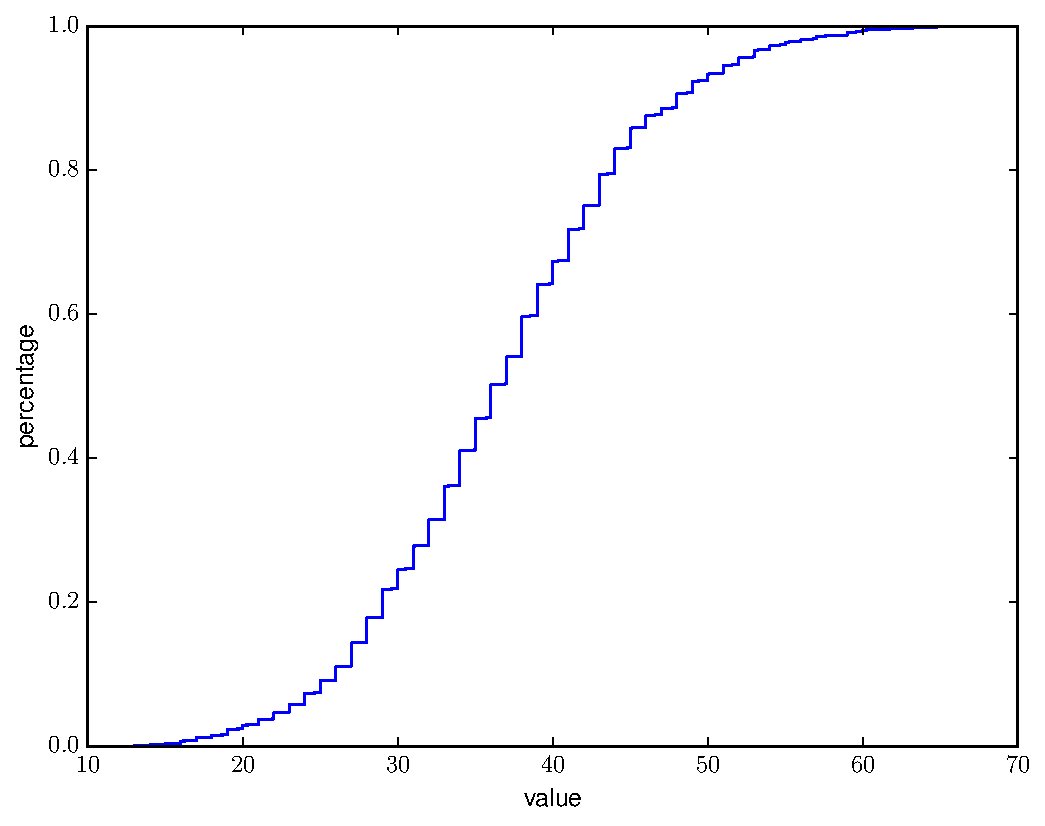
\includegraphics[width=.75\textwidth]{prob2b.pdf}
\end{figure}

Code for the multiple runs: 

\begin{lstlisting}[language=Python]
def RandomVals(l,d):
    return 1.0/np.sqrt(l) * np.asarray([normal() for i in range(d)])

l_vals = []
for i in range(1000):
    l = 0

    A_ = norm(A)**2/10
    err = norm(A)**2
    while err > A_:
        l += 1
        S = [RandomVals(l, np.shape(A)[0]) for i in range(l)]    
        S = np.asarray(S)
        B = np.dot(S, A)
        err = norm(np.dot(A.T, A) - np.dot(B.T, B))
    l_vals.append(int(l))

l_vals = np.asarray(np.sort(l_vals))
l_ = l_vals/(0.1 * l_vals.sum())
l_ = np.cumsum(l_ * 0.1)
\end{lstlisting}


%%%%%%%%%%%%%%%%%%%%%%%%%%%%%%%%%%%%%%%%%%%%%%%%%%%%
%%%%%%%%%%%%%%%%%%%%%%%%%%%%%%%%%%%%%%%%%%%%%%%%%%%%
%%%%%%%%%%%%%%%%%%%%%%%%%%%%%%%%%%%%%%%%%%%%%%%%%%%%
\section{Linear Regression (40 points)}

We will find coefficients \texttt{C} (was $a_1, \ldots, a_d$ in notes, but changed to avoid confusion with matrix \texttt{A} in {\bf{\sffamily Q1}}) to estimate \texttt{X*C $\approx$ Y}, using the provided datasets \texttt{X} and \texttt{Y}.  We will compare two approaches \emph{least squares} and \emph{ridge regression}.  

\begin{itemize} \denselist
\item[\textsf{Least Squares:} ]  Set \texttt{C = inverse(X' * X)*X'*Y}
\item[\textsf{Ridge Regression:} ] Set \texttt{Cs = inverse(X'*X + s\^{}2*eye(12))*X'*Y}
\end{itemize}

\paragraph{A (20 points): }
Solve for the coefficients \texttt{C} (or \texttt{Cs}) using Least Squares and Ridge Regression with $s = \{0.1, 0.3, 0.5, 1.0, 2.0\}$ (i.e. $s$ will take on one of those $5$ values each time you try, say obtaining \texttt{C05} for $s=0.5$).  
For each set of coefficients, report the error in the estimate $\hat{Y}$ of $Y$ as 
\texttt{norm(Y - X*C,2)}.

\ \newline
\ \newline

{\em Note:} Least Squares is the same as Ridge Regression with $s = 0$, so $s=0$ denotes the results for the Least Squares Method.

\begin{table}[H]
\centering
\begin{tabular}{@{}l r@{}}
\hline\hline
$s$ & $\left|\left| Y - X\cdot C\right|\right|_{2}$\\
\hline
0.0 & 25.8245 \\
0.1 & 25.8245 \\
0.3 & 25.8246 \\
0.5 & 25.8248 \\
1.0 & 25.8289 \\
2.0 & 25.8943 \\
\hline
\end{tabular}
\end{table}


\paragraph{B (20 points): }
Create three row-subsets of \texttt{X} and \texttt{Y}
\begin{itemize} \denselist
\item \texttt{X1 = X(1:66,:)} and \texttt{Y1 = Y(1:66)}
\item \texttt{X2 = X(34:100,:)} and \texttt{Y2 = Y(34:100)}
\item \texttt{X3 = [X(1:33,:); X(67:100,:)]} and \texttt{Y3 = [Y(1:33); Y(67:100)]}
\end{itemize}

Repeat the above procedure on these subsets and \emph{cross-validate} the solution on the remainder of \texttt{X} and \texttt{Y}.  Specifically, learn the coefficients \texttt{C} using, say, \texttt{X1 and Y1} and then measure \texttt{norm(Y(67:100) - X(67:100,:)*C,2)}.  

Which approach works best (averaging the results from the three subsets): Least Squares, or for which value of $s$ using Ridge Regression?  

\begin{table}[H]
\centering
\caption{$(X_{1},\ Y_{1})$}
\begin{tabular}{@{}l r@{}}
\hline\hline
$s$ & $\left|\left| Y - X\cdot C\right|\right|_{2}$\\
\hline
0.0 & 14.7834 \\
0.1 & 14.7815 \\
0.3 & 14.7666 \\
0.5 & 14.7370 \\
1.0 & 14.6027 \\
2.0 & 14.1411 \\
\hline
\end{tabular}
\end{table}

\begin{table}[H]
\centering
\caption{$(X_{2},\ Y_{2})$}
\begin{tabular}{@{}l r@{}}
\hline\hline
$s$ & $\left|\left| Y - X\cdot C\right|\right|_{2}$\\
\hline
0.0 & 14.5124 \\
0.1 & 14.5129 \\
0.3 & 14.5173 \\
0.5 & 14.5263 \\
1.0 & 14.5734 \\
2.0 & 14.8370 \\
\hline
\end{tabular}
\end{table}

\begin{table}[H]
\centering
\caption{$(X_{3},\ Y_{3})$}
\begin{tabular}{@{}l r@{}}
\hline\hline
$s$ & $\left|\left| Y - X\cdot C\right|\right|_{2}$\\
\hline
0.0 & 23.1627 \\
0.1 & 23.1633 \\
0.3 & 23.1686 \\
0.5 & 23.1794 \\
1.0 & 23.2336 \\
2.0 & 23.5070 \\
\hline
\end{tabular}
\end{table}

As the above tables show, the first two instances of the data converge the best. Also, it's important to note that the best values of convergence occur for $s \ll 1$, which makes sense as this is the regularized normal equation that we're using in ridge regression. The best results occur from using ridge regression with $s = 0.1$.

%%%%%%%%%%%%%%%%%%%%%%%%%%%%%%%%%%%%%%%%%%%%%%%%%%%%
%%%%%%%%%%%%%%%%%%%%%%%%%%%%%%%%%%%%%%%%%%%%%%%%%%%%
%%%%%%%%%%%%%%%%%%%%%%%%%%%%%%%%%%%%%%%%%%%%%%%%%%%%


\end{document}
